\chapter{Lepton Flavour in the Standard Model and Beyond}\label{chapter1}

% \begin{markdown}
% ---

% + Yoshi said: this is really an intro to CLFV searches for experts out of the
% field.

% + What's a muon?
% + What does the SM predict muons can/can't do
% + Historical context, motivation
%  + Why/how was the first CLFV experiment conducted?

% Sindrum II: what do they start with?
%  - Generation mixing in neutrino oscillations


% ---
% \end{markdown}

% v1
The Standard Model (SM) of particle physics is possibly the most successful
mathematical model of physical phenomena so far. It provides accurate
predictions for all observable interactions between known elementary particles.

% The very start of this chapter should introduce HEP concepts like the muon and
% what it is, how it relates to the SM, what is the SM.

% This thesis concerns itself with addressing some of the challenges faced in the
% simulation of particles within the experimental setup of the COMET experiment.

% However before we are able to dive into the main topics, it is necessary to
% discuss the purpose of the experiment, how it emerges from the current state of
% our knowledge of elementary particle physics, and the steps taken to get there.


% v0
% Explain the SM. Something like
% The Standard Model is the theory at the heart of modern particle physics. Built
% upon special relativity and quantum mechanics, it describes the interactions
% between elementary particles and allows physicists to predict the outcome of
% interactions and decays to a previously unattainable precision. Little evidence
% so far has been able to contradict the formulation of the Standard Model,
% despite many fundamental questions remaining unanswered, such as the nature of
% dark matter, the reason for the matter-antimatter asymmetry in the universe, or
% the existence of exactly three generations of leptons and quarks.


\section{Discovery of the muon}
The first traces of muons were observed around 1937 by three experiments
investigating the nature of cosmic ray-induced particle
showers~\cite{PhysRev.51.884, PhysRev.52.1198, PhysRev.52.1003}. 
In addition, one analysis was able to estimate the mass of the discovered
particle at 130 times that of the electron. 
In 1935, Yukawa predicted the existence of a particle with a similar mass whose role
was to carry the strong force and bind atomic nuclei
together~\cite{10.1143/PTPS.1.1}. Hence the muon and Yukawa's particle were
originally believed to be one and the same particle, and it was only when
Yukawa's meson (now called $\pi$, for primary) was observed decaying into a muon,
that the two particles were completely disambiguated~\cite{LATTES1947}.

It was the fact that the muon appeared as nothing but a heavy electron which
prompted Rabi to ask ``who ordered that?'' in response to its discovery. In
fact, the Standard Model still cannot give a satisfactory answer to this
question as it does not motivate the existence of three generations of
elementary particles. As far as the SM can explain, there is no fundamental reason
for the existence of heavier or lighter versions of particles that share the
same quantum properties.

\section{The muon in the Standard Model}
The SM identifies the muon as the second-generation charged lepton, meaning it
is a fermion with identical quantum numbers (aside from flavour) as the electron
and tau lepton. The only way for a muon to decay in a vacuum is through the weak
force. The diagram for muon decay is shown in Fig.~\ref{fig:weak_decay}.

\begin{figure}
    \centering
    %\includegraphics[]{}
    \caption{Feynman diagram for the weak decay of the muon.}
    \label{fig:weak_decay}
\end{figure}




% Allowed and forbidden decays

% g-2 measurement
\cite{PhysRevLett.126.141801} % g-2

% Is lhc-b related here? Lepton univ?
\cite{lhcbcollaboration2021test} % lhc-b R_K




\section{Charged lepton flavour violation}
Quark generations are known to mix

\begin{figure}
    \centering
    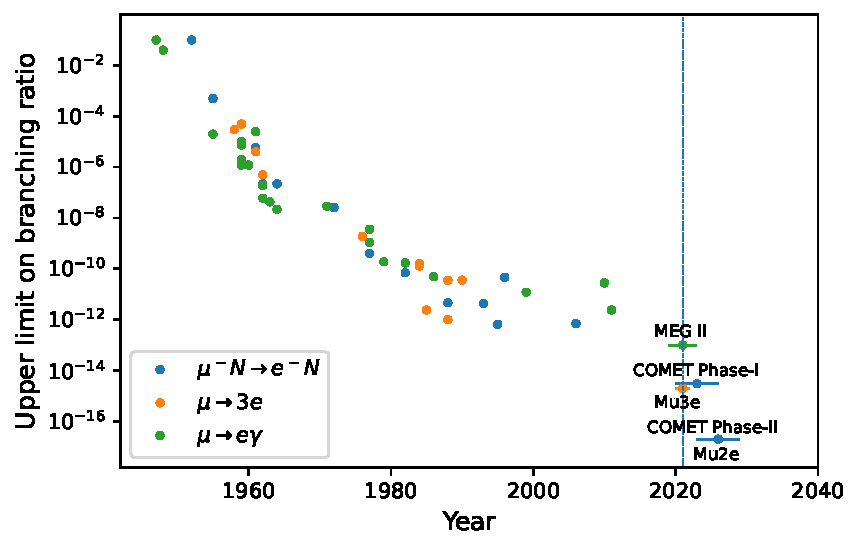
\includegraphics{chapter1/clfv_upper_limit.pdf}
    \caption{90\%-confidence upper limit on the branching ratio of three charged lepton flavour-violating processes over time. The past data points were tabulated in~\cite{BERNSTEIN201327}. Future data points are the expected sensitivities quoted in the MEG II~\cite{Baldini2018}, Mu3e~\cite{ARNDT2021165679}, COMET Phase-I~\cite{the_comet_collaboration_comet_2020} and Mu2e~\cite{bartoszek2015mu2e} design reports.}
    \label{fig:clfv_upper_limit}
\end{figure}

%The search for Lepton Flavour Violation started in 19XX with John Doe's experiment~\cite{doe}.



%See Chapter~\ref{chapter2}, read~\cite{goodfellow_generative_2014}.\\
%The smooth boi can be seen on Fig.~\ref{subfig:smooth_boi}, and the outlined boi on %Fig.~\ref{subfig:smooth_boi}. The whole figure is Fig.~\ref{fig:my_label}.
%
%A derivative:
%$$\diff{x}{y} = 2\pi x y$$
%Insane!
%
%And here we typeset COMET in smallcaps: \COMET. This \acrshort{COMET} is an \emph{acronym}. %You can click it to see what it means.
%
%\begin{figure}
%    \centering
%    \subfloat[A smooth boi]{
%    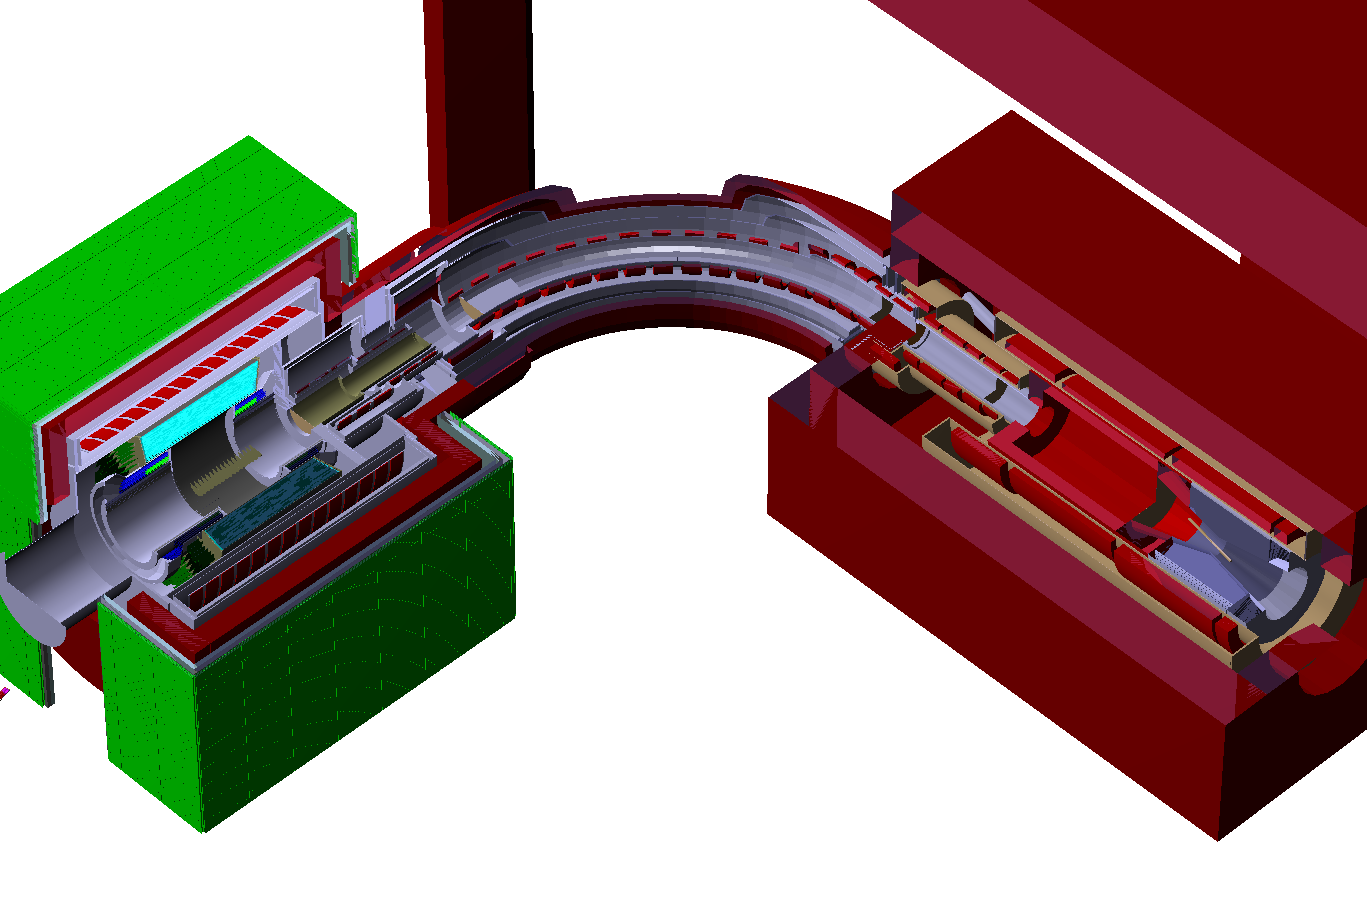
\includegraphics[width=0.5\textwidth]{viewer_smooth.png}
%    \label{subfig:smooth_boi}
%    }
%    \subfloat[An outlined boi]{
%    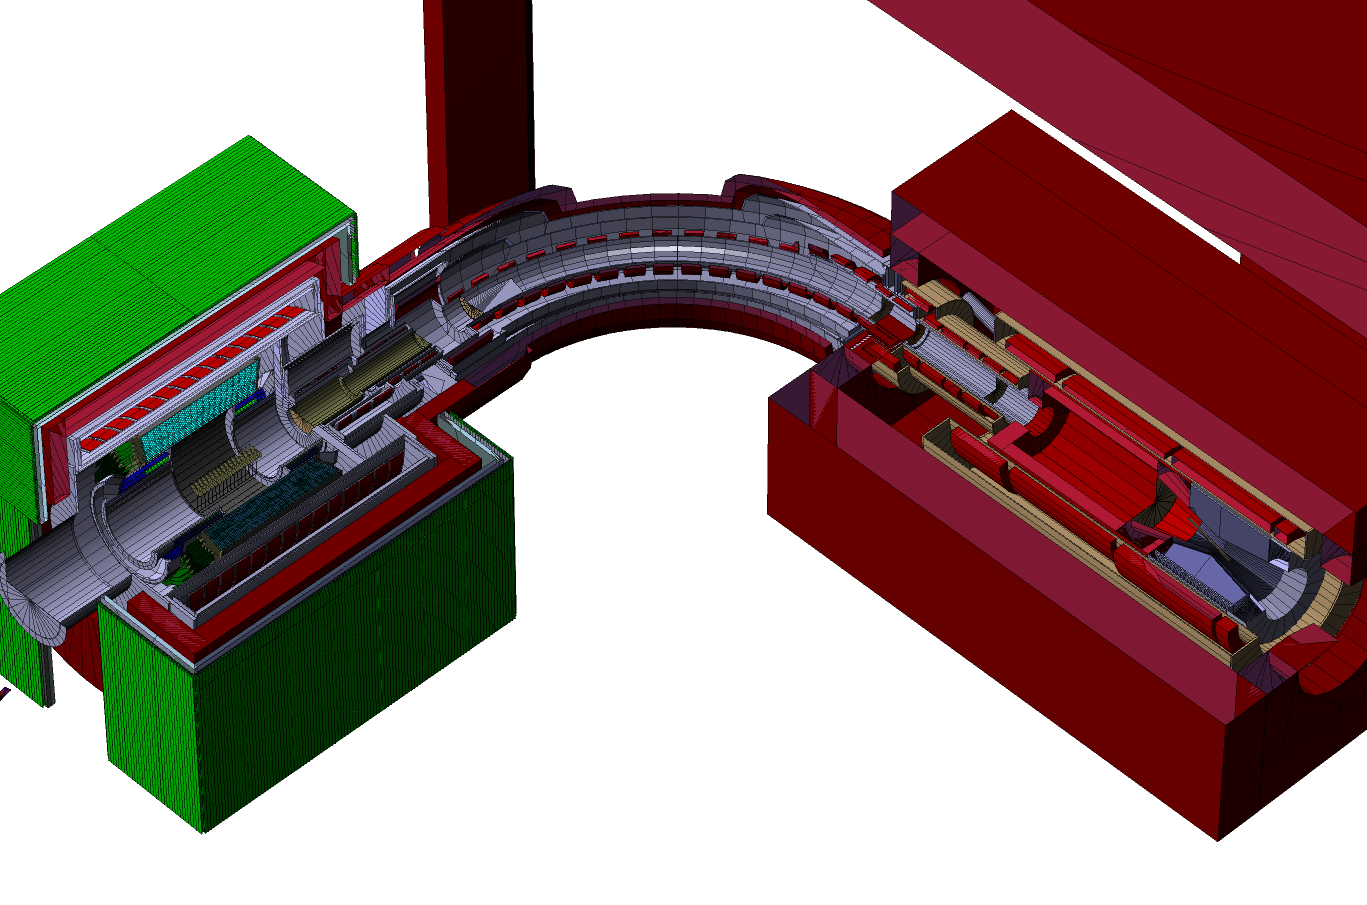
\includegraphics[width=0.5\textwidth]{viewer_outline2.png}
%    \label{subfig:outlined_boi}
%    }
%    \caption{Phase-I cutaway geometries.}
%    \label{fig:my_label}
%\end{figure}
%
%Here we cite the COMET TDR~\cite{the_comet_collaboration_comet_2020} and the upper limit on %the branching ratio of $\mu^- + \textrm{Al} \rightarrow e^- + \textrm{Al}$, $7\times %10^{-13}$, by the SINDRUM-II experiment~\cite{Bertl:2006up}.
